\documentclass[11pt]{article}
\usepackage[utf8]{inputenc}
\usepackage{graphicx}
\usepackage{booktabs}
\usepackage{caption}
\usepackage{subcaption}
\usepackage{geometry}
\geometry{margin=1in}

\title{Comparison of DQN Architectures on CartPole-v1}
\author{CleanRL Models}
\date{}

\begin{document}
\maketitle

\section{Architectures}

All models use the same training setup: 500k steps, Adam (lr $2.5\times10^{-4}$), buffer 10k, $\gamma=0.99$, batch 128.

\begin{table}[h]
\centering
\caption{Network architectures (CartPole: obs dim 4, 2 actions).}
\begin{tabular}{@{}llc@{}}
\toprule
Model & Architecture & Activations \\
\midrule
dqn\_original & obs $\to$ 120 $\to$ 84 $\to$ actions & ReLU after each hidden layer \\
dqn\_3layers & obs $\to$ 120 $\to$ actions & ReLU after hidden layer \\
dqn\_linear & obs $\to$ 120 $\to$ actions & none (1 hidden, all linear) \\
dqn\_4layers\_linear & obs $\to$ 120 $\to$ 84 $\to$ actions & none (all linear) \\
\bottomrule
\end{tabular}
\end{table}

\section{Results}

Training dashboards (episode return, TD loss, mean Q) for each model. Same hyperparameters; only the Q-network architecture differs.

\begin{figure}[htbp]
\centering
\begin{subfigure}[b]{0.48\textwidth}
  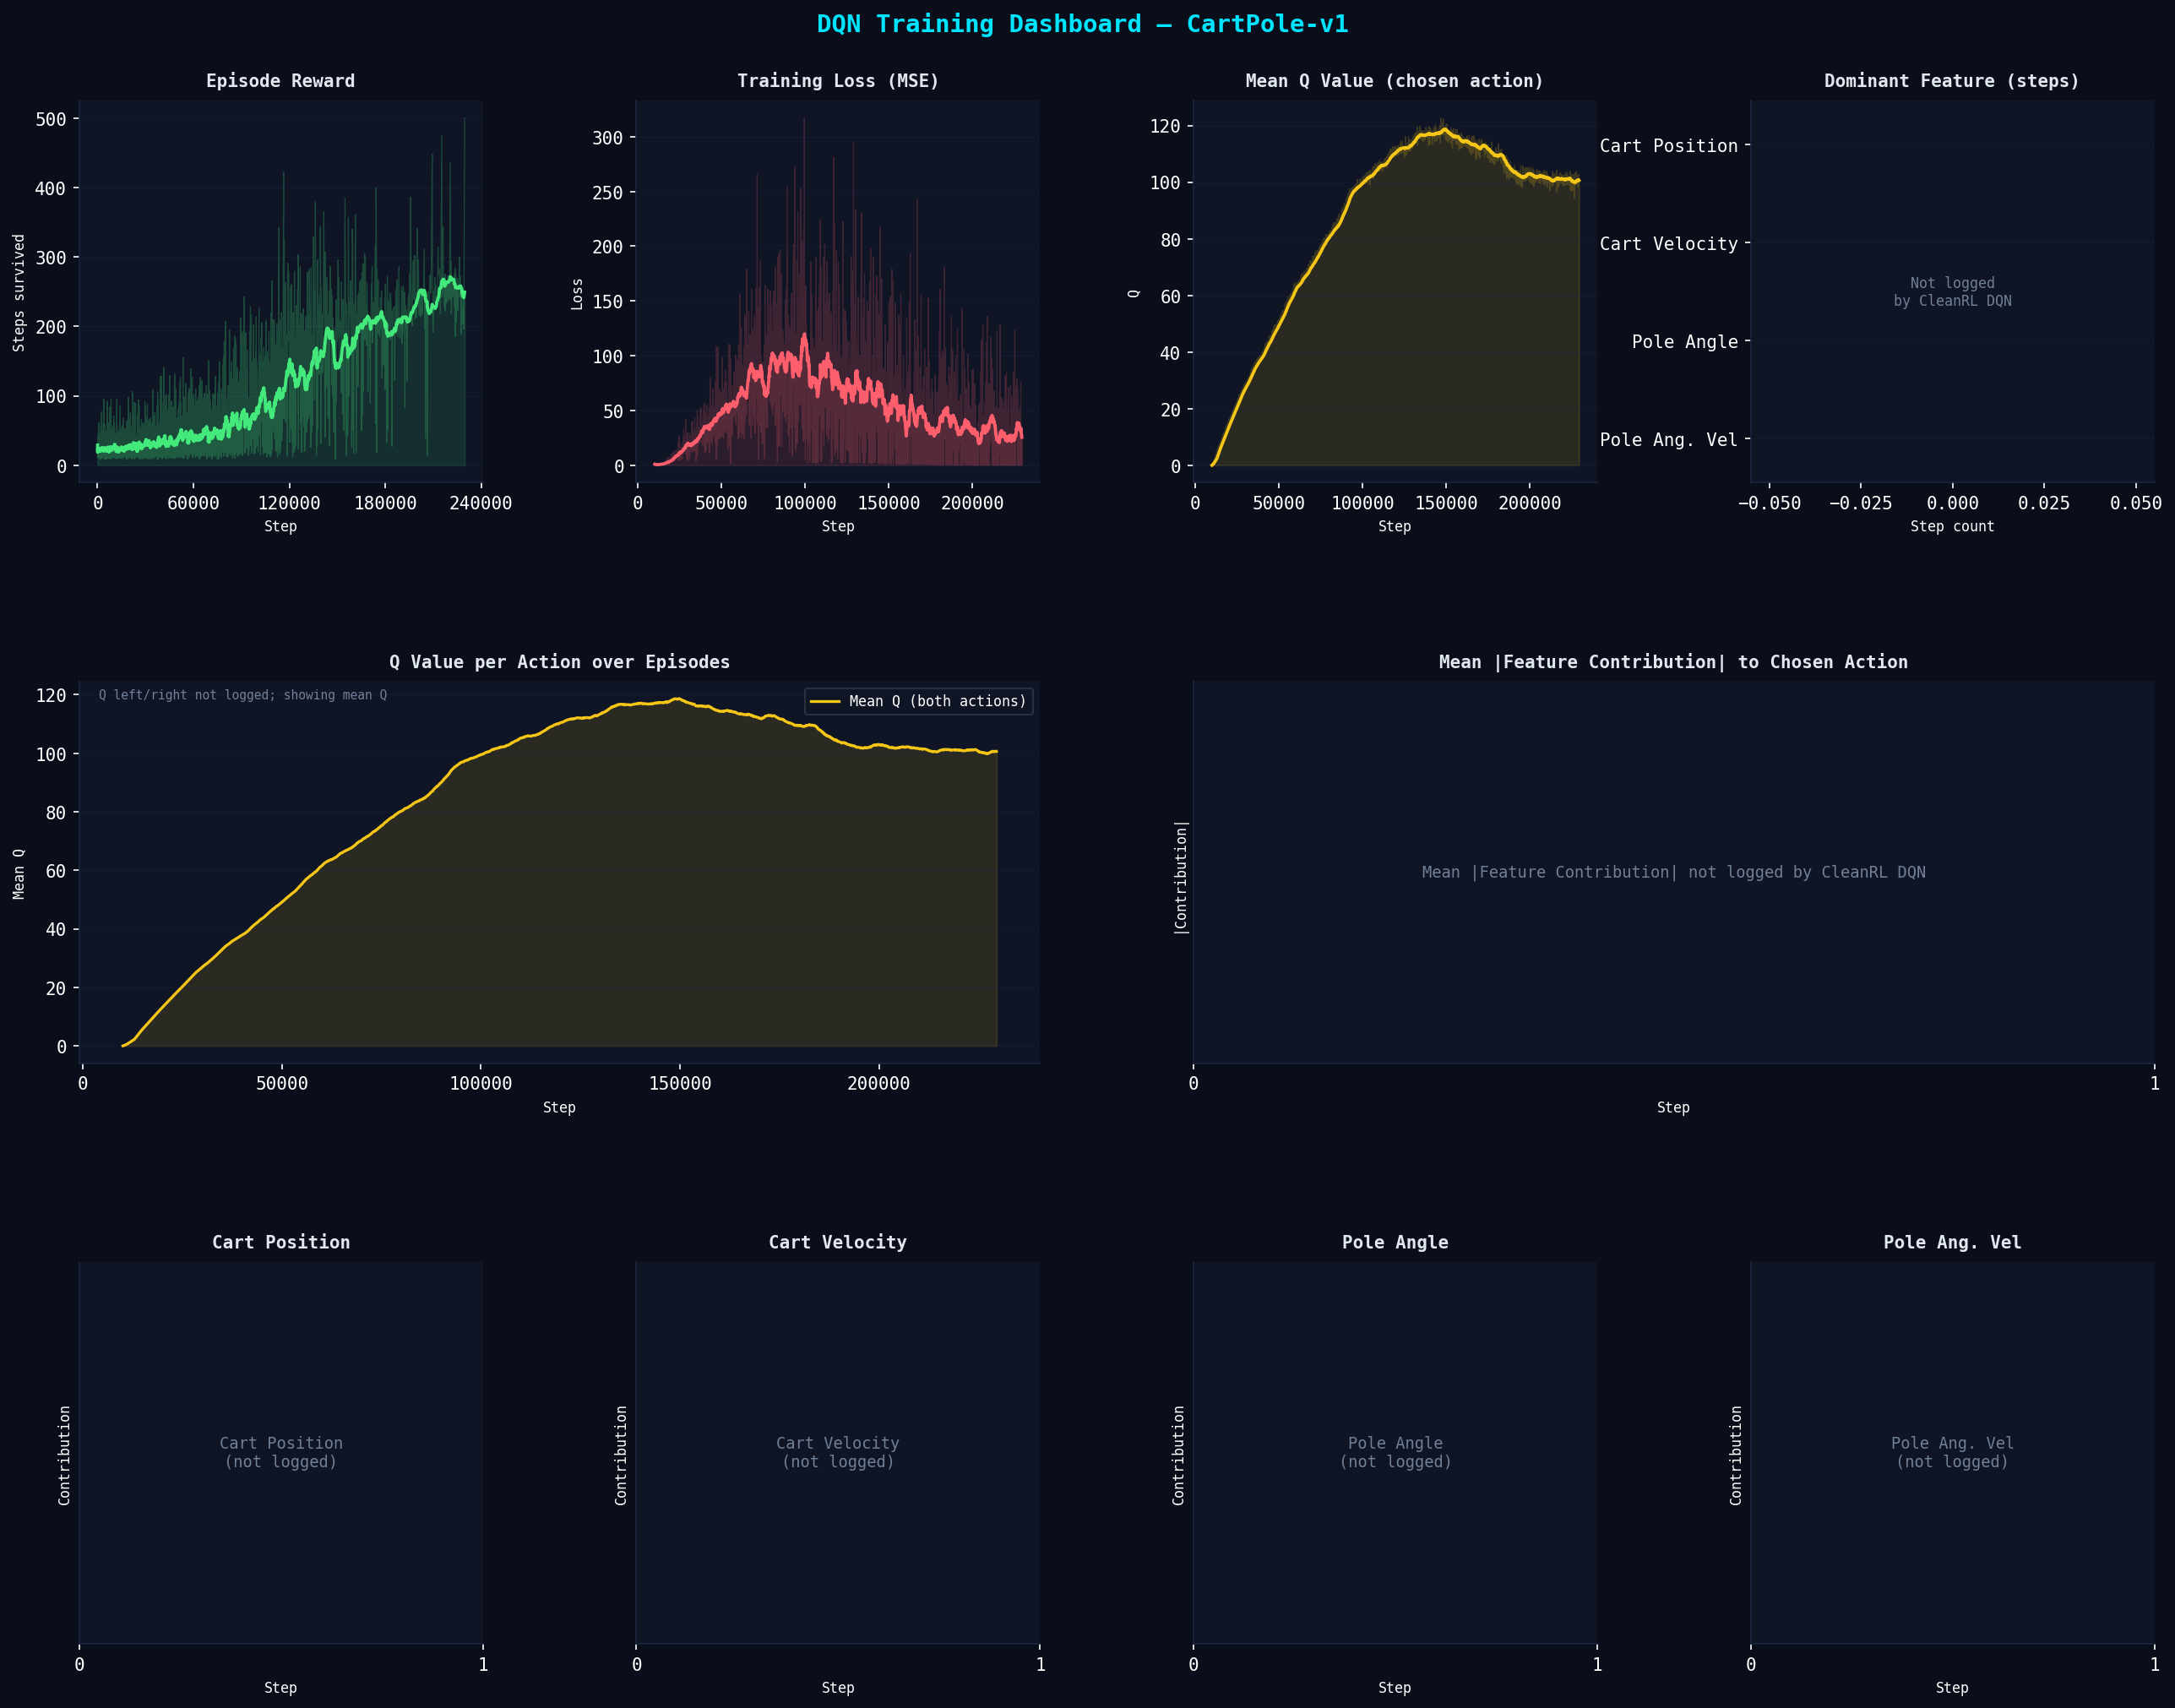
\includegraphics[width=\textwidth]{figures/dqn_original.png}
  \caption{dqn\_original (2 hidden, ReLU)}
\end{subfigure}
\hfill
\begin{subfigure}[b]{0.48\textwidth}
  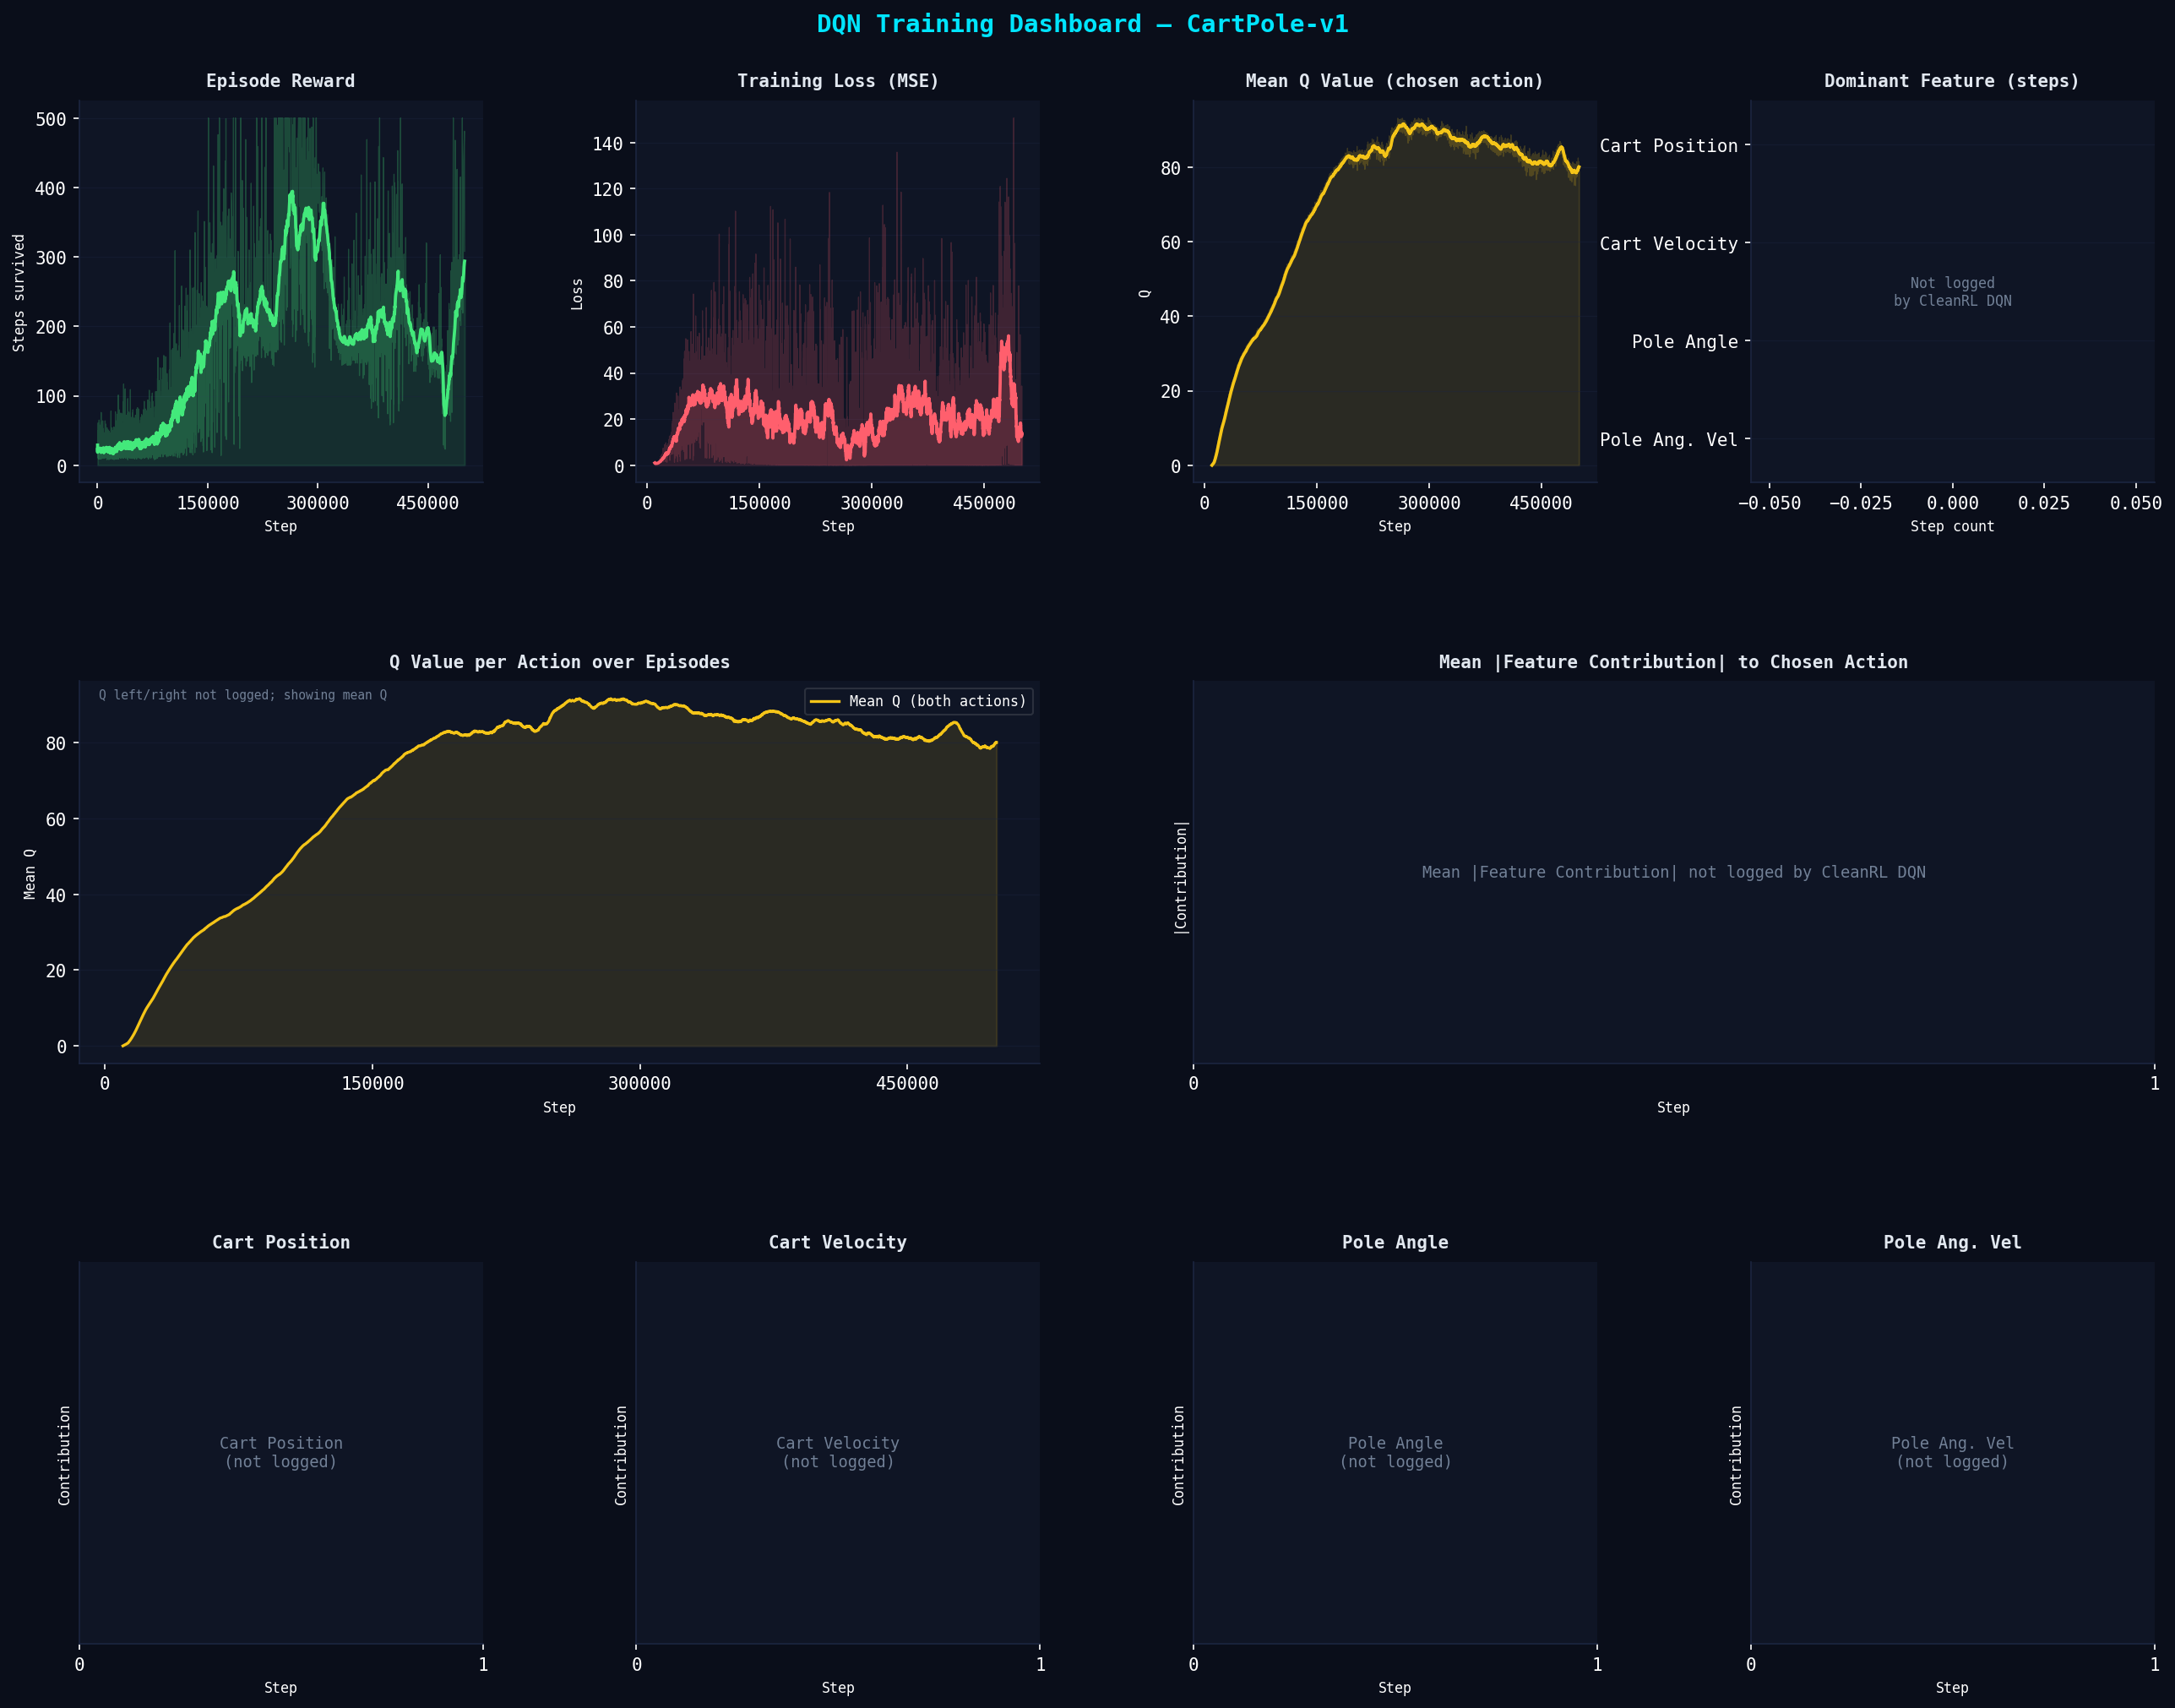
\includegraphics[width=\textwidth]{figures/dqn_3layers.png}
  \caption{dqn\_3layers (1 hidden, ReLU)}
\end{subfigure}

\vspace{1em}
\begin{subfigure}[b]{0.48\textwidth}
  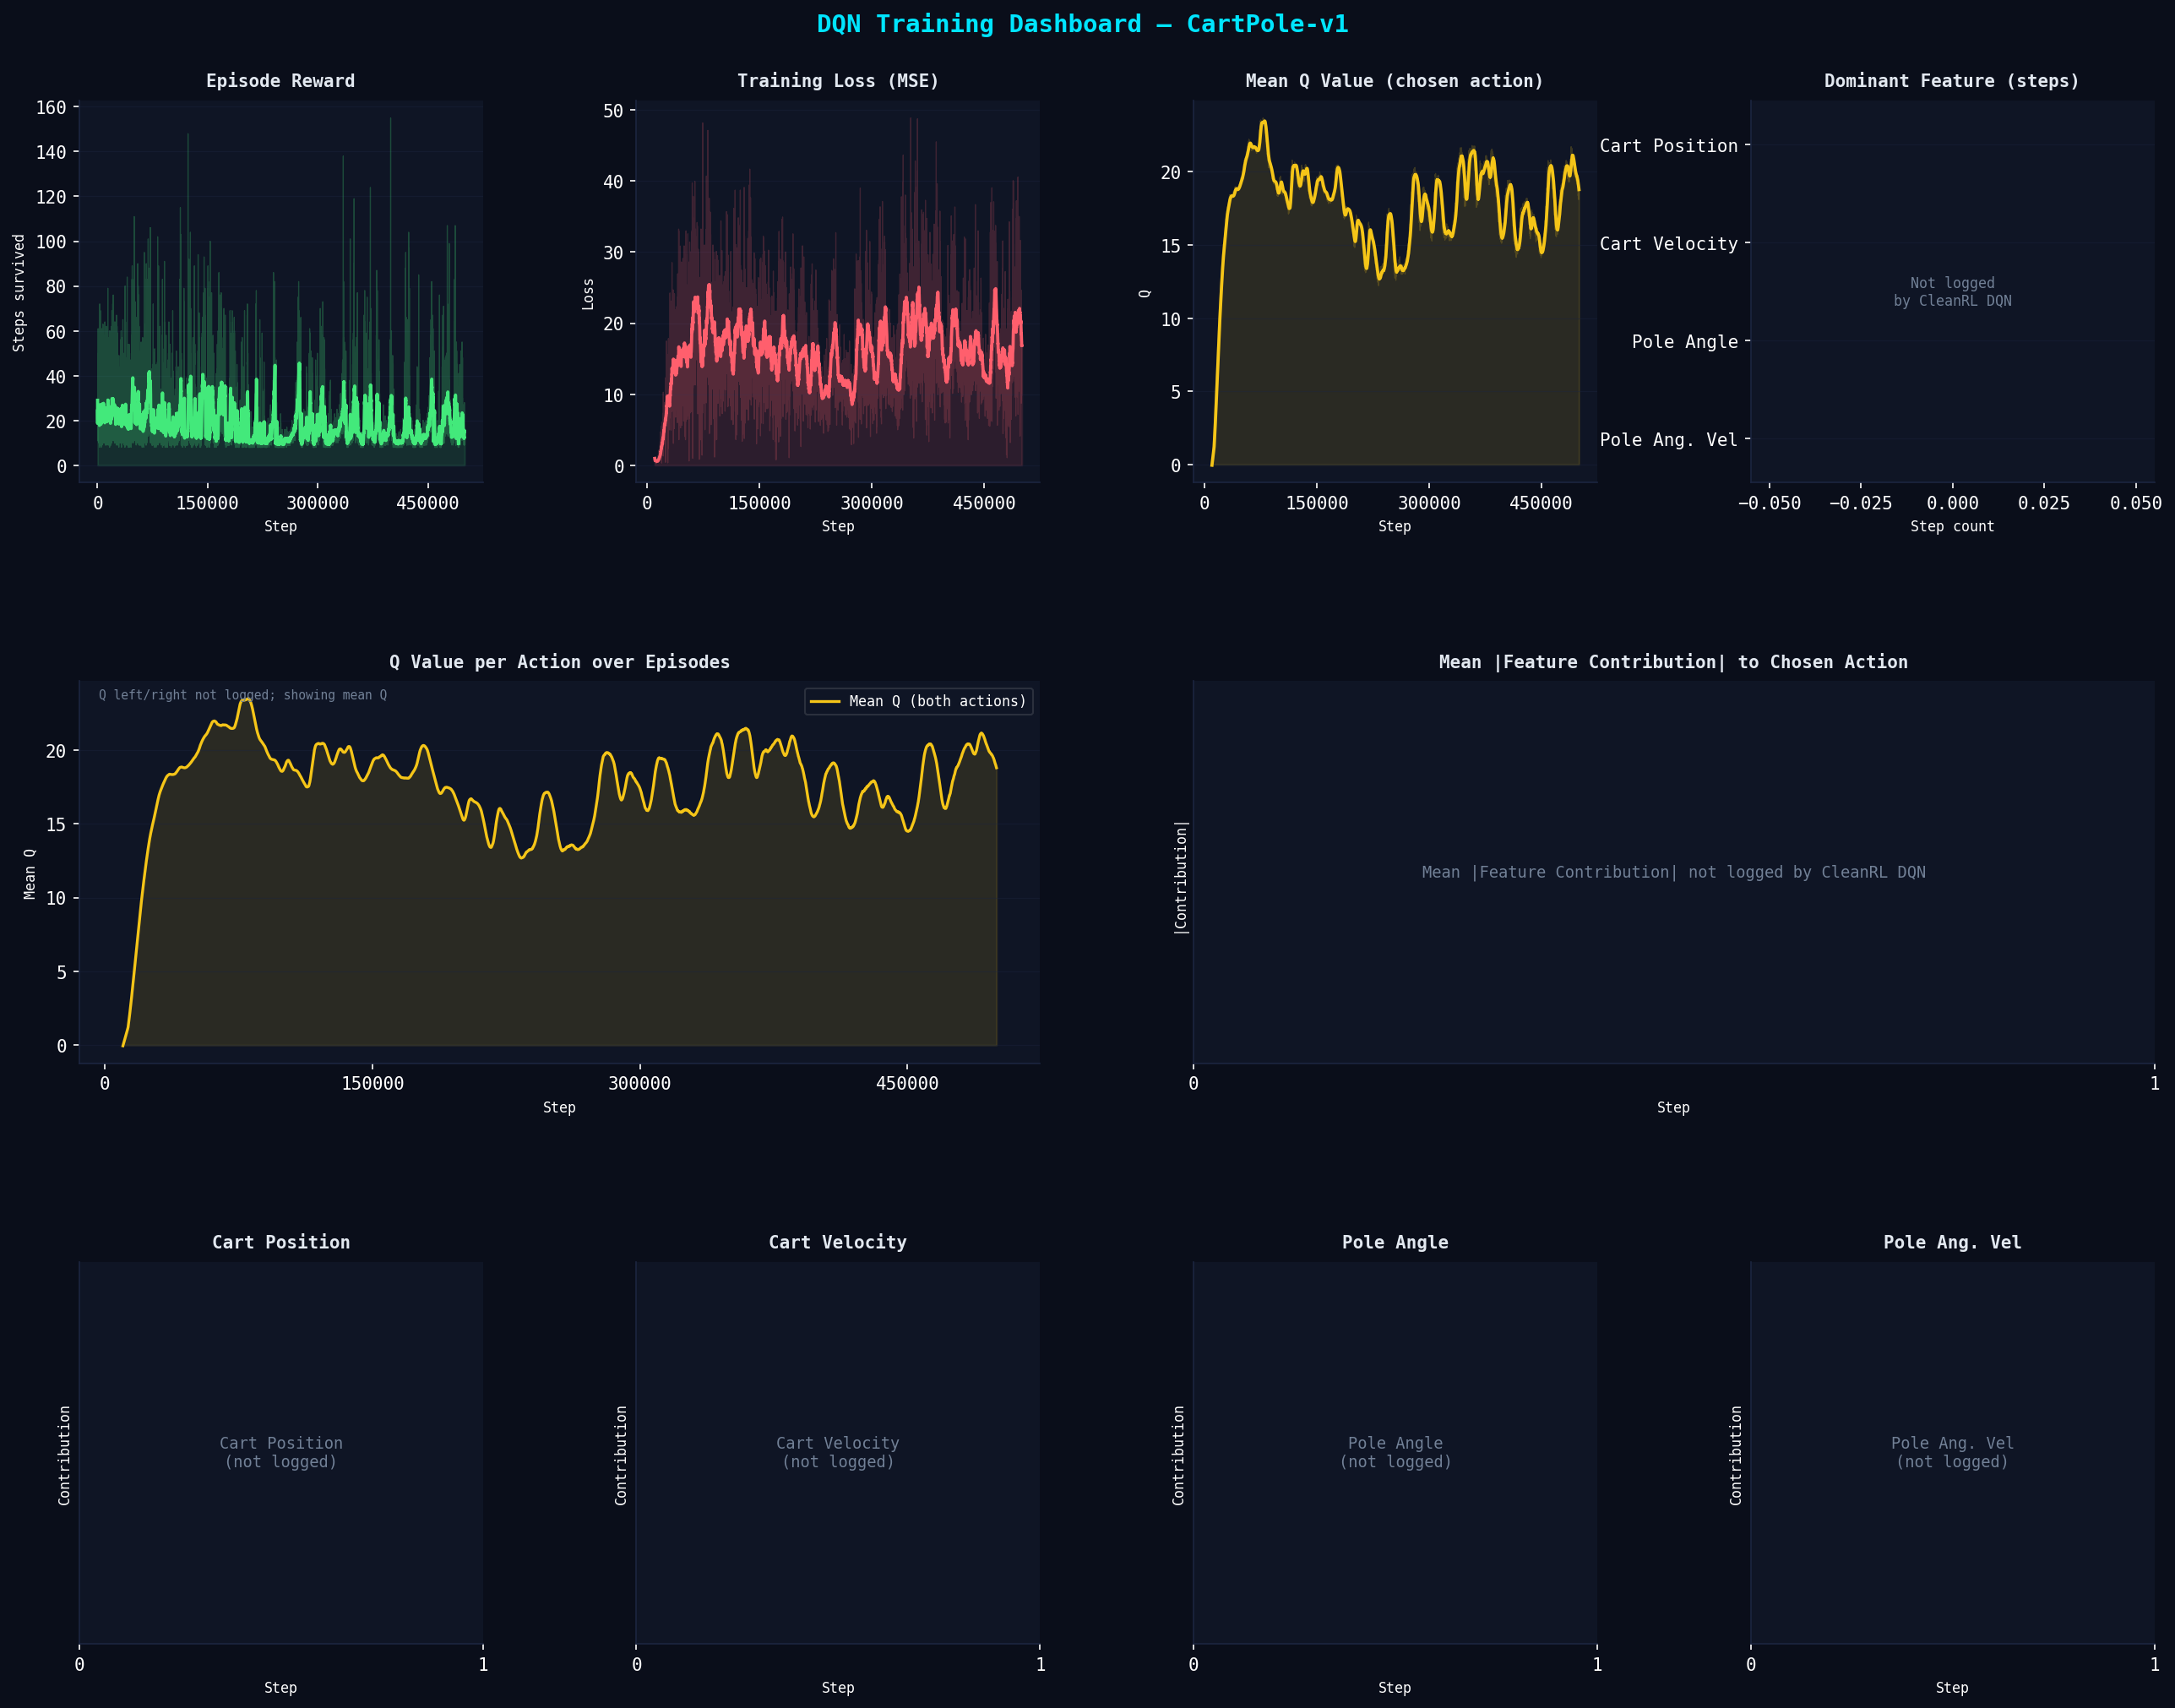
\includegraphics[width=\textwidth]{figures/dqn_linear.png}
  \caption{dqn\_linear (1 hidden, linear only)}
\end{subfigure}
\hfill
\begin{subfigure}[b]{0.48\textwidth}
  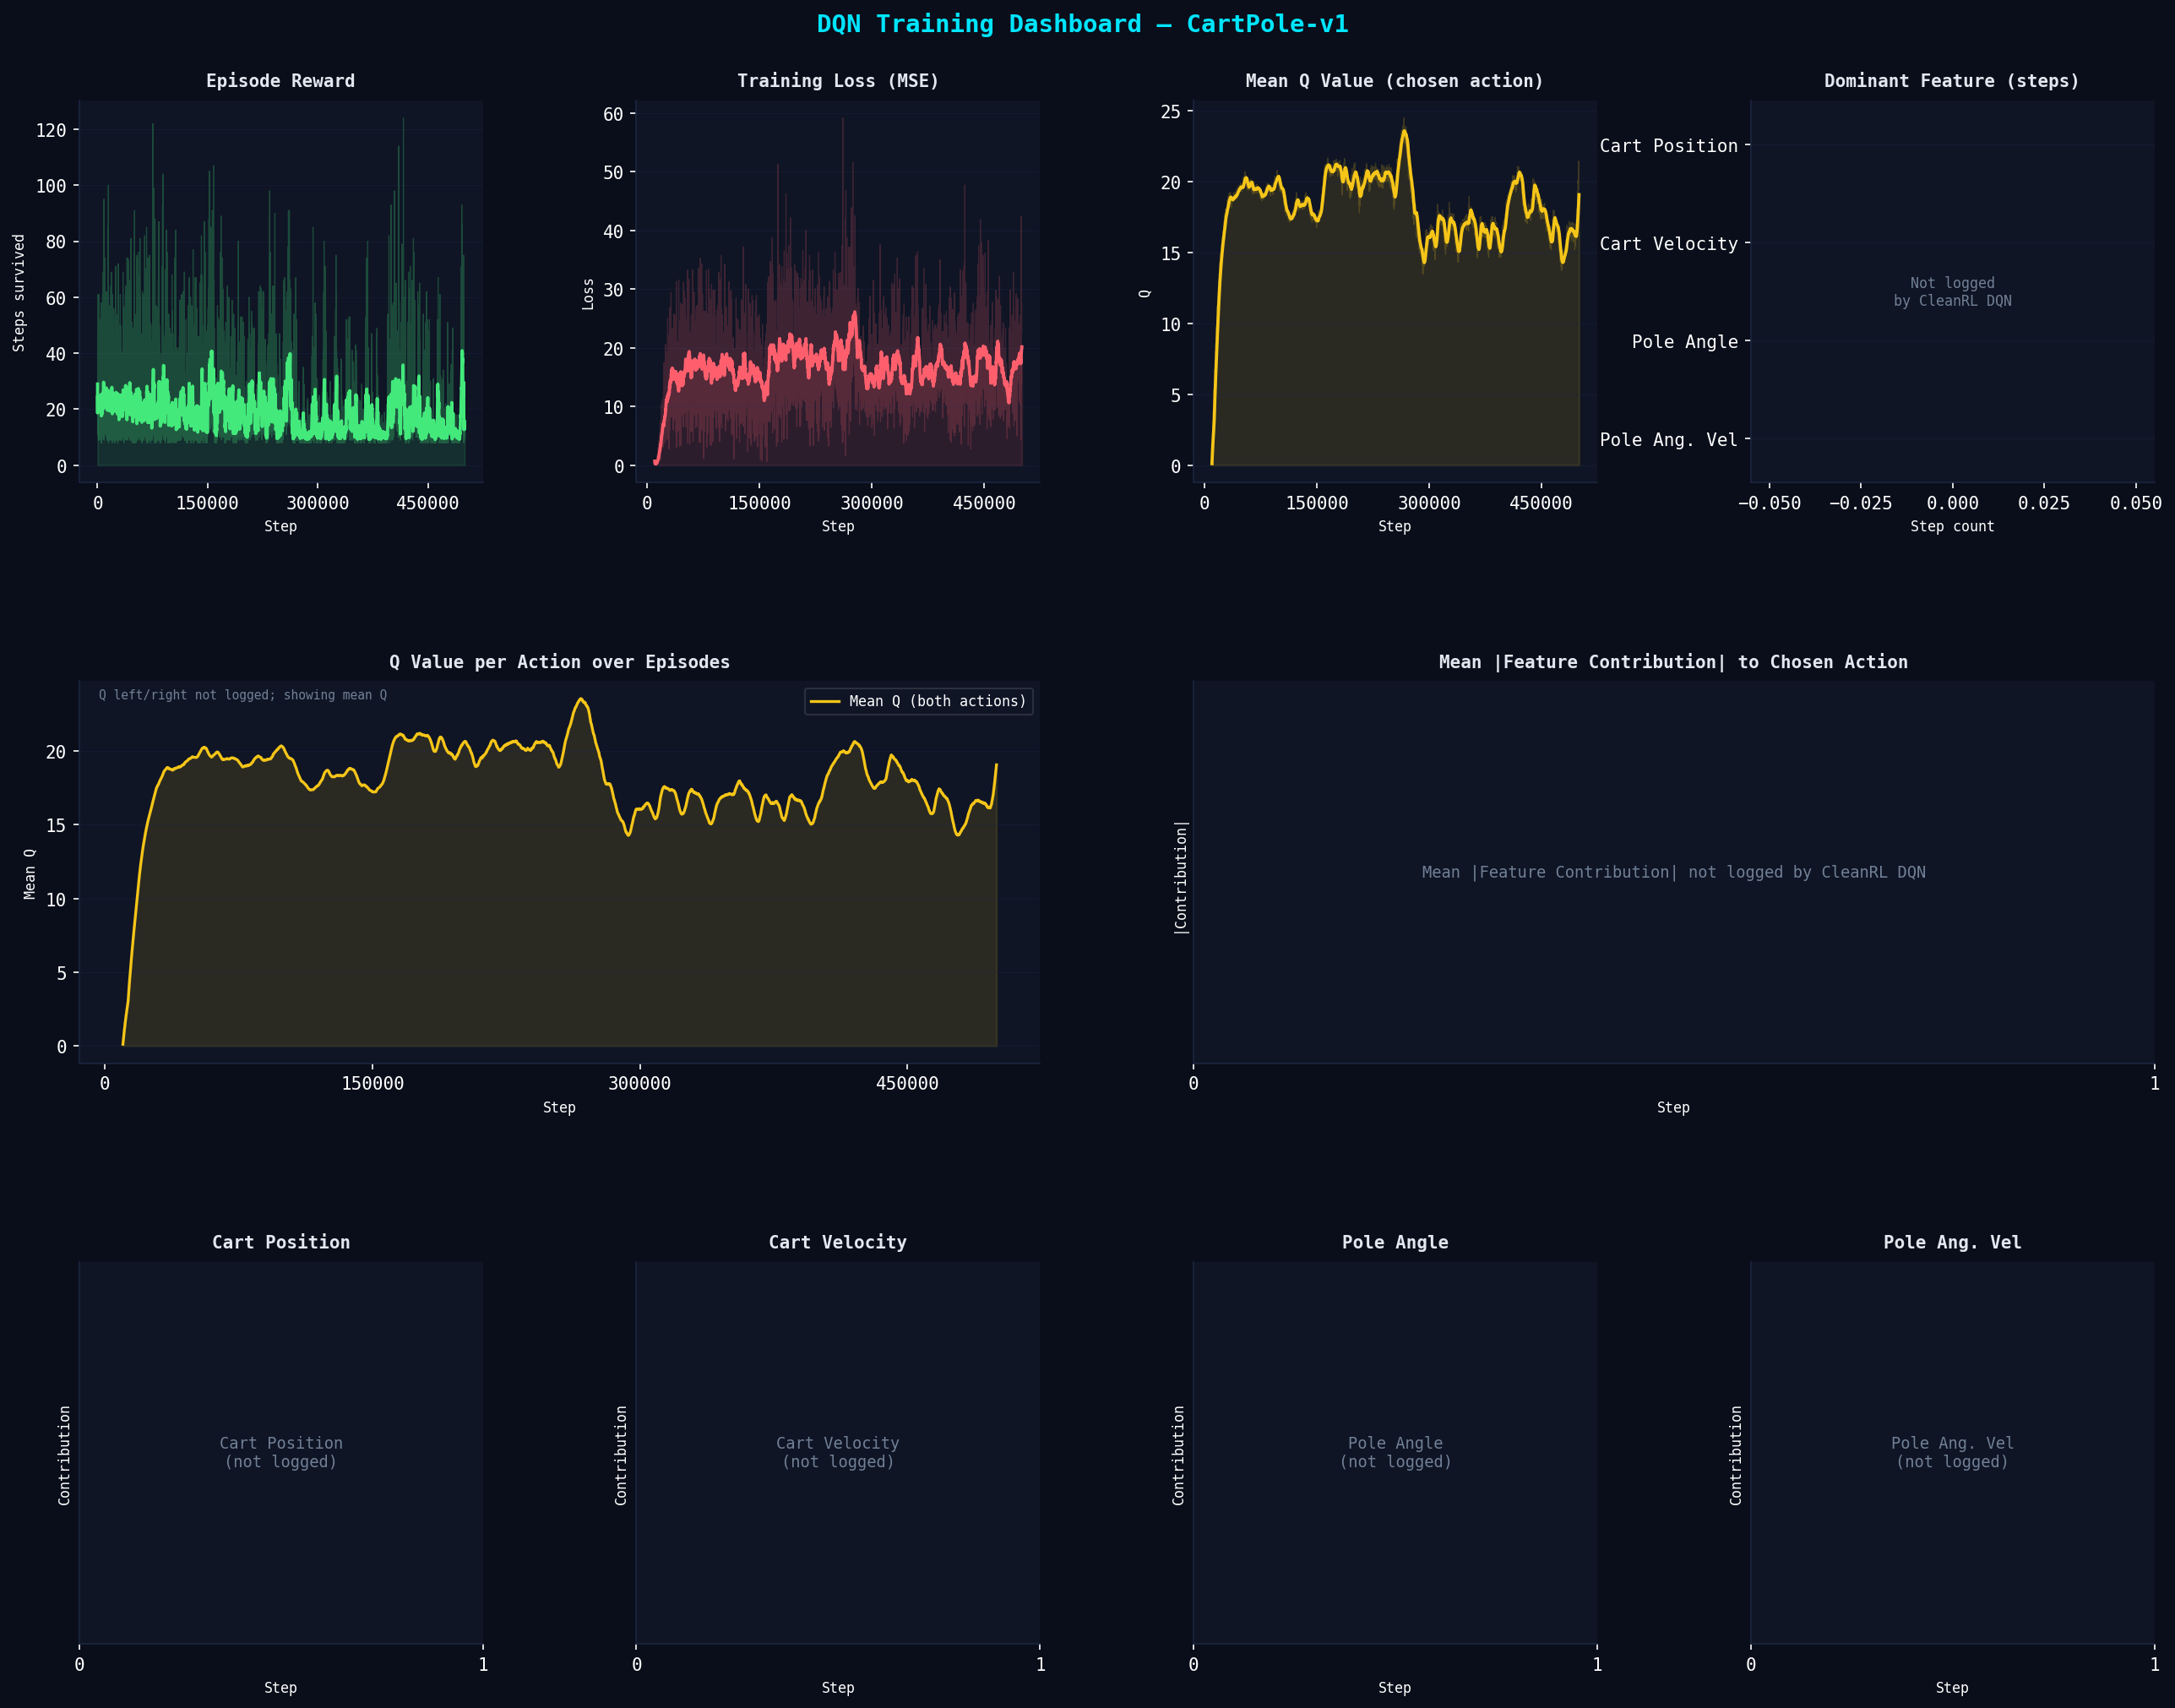
\includegraphics[width=\textwidth]{figures/dqn_4layers_linear.png}
  \caption{dqn\_4layers\_linear (2 hidden, linear only)}
\end{subfigure}
\caption{DQN training dashboards on CartPole-v1 (500k steps).}
\end{figure}

\section{Summary}

\begin{itemize}
  \item \textbf{dqn\_original}: Full DQN (2 hidden layers + ReLU); typically learns well and reaches high episodic return.
  \item \textbf{dqn\_3layers}: One hidden layer + ReLU; fewer parameters, often similar performance to original.
  \item \textbf{dqn\_linear}: One hidden layer (120), all linear; no ReLU, equivalent to one linear map but with more parameters than single-layer linear.
  \item \textbf{dqn\_4layers\_linear}: Same shape as original but no ReLU; equivalent to one linear map, usually worse than ReLU version.
\end{itemize}

\end{document}
